\section{Problems}

\noindent {\bf Problem \thesection.\theprob}\stepcounter{prob}

Calculate the hydraulic power of the double-acting piston pump, which delivers water from an open-surface tank into a closed one with $500[kPa]$ gauge pressure (i.e. relative pressure) located $50[m]$ above the suction tank. Diameter of the piston is $D=120[mm]$, the stroke is $150[mm]$ and the driving motor runs at $120[rpm]$.

\emph{Solution:} 

$Q_{mean}=2 \times A_{piston} \times s \times n=2\times \frac{0.12^2 \pi}{4} \times 0.15 \times \frac{120}{60} =6.78 \times 10^{-3} [\frac{m^3}{s}]$

$\Delta p=p_{tank,abs.}-p_0\,+\,\rho g H=p_{tank,rel.}\,+\,\rho g H=991[kPa]$

$P=Q \Delta p=6.72[kW]$

%%%%%%%%%%%%%%%%%%%%%%%%%%%%%%%%%%%%%%%%%%%%%%%%%%%%

\vspace{1cm}
\noindent {\bf Problem \thesection.\theprob}\stepcounter{prob}

The characteristic curve of a gear pump is $Q[dm^3/min]=11.93-0.0043 \Delta p [bar]$. The volumetric efficiency at $35 bar$ pressure difference is $92\%$. Find the volume flow rate and the geometric volume! The shaft speed is $80 rev/min$. How large is the driving torque if the pump efficiency is $85\%$? (Solution: $Q=11.78\,dm^3/min$, $V_g = 160\,cm^3$, $M = 96.5\,Nm$)

%%%%%%%%%%%%%%%%%%%%%%%%%%%%%%%%%%%%%%%%%%%%%%%%%%%%

\vspace{1cm}
\noindent {\bf Problem \thesection.\theprob}\stepcounter{prob}

The piston diameter of a hydraulic cylinder is $50 mm$. An $800 kg$ load is lifted by the piston rod of $20 mm$ diameter with $12 m/min$ velocity. How large must be the flow rate $Q$ of the gear pump rotating with $n = 960/min$ speed if its volumetric efficiency is $92\%$? Find the geometric volume of the pump and the pressure rise produced by it! Find the power $P$ and the torque $M$ of the driving motor! The pump efficiency is $74\%$. Prepare a sketch of the gear pump showing the rotation direction of the shafts, intake and delivery ports! How large will be $P’$, $M$, $Q’$ if the rotor speed is $n’ = 1440/min$? (Solution: $Q_g = 21.5\,dm^3/min$, $V_g = 22.4\,cm^3$, $\Delta p = 47.6\,bar$, $P=2.12\,kW$, $M=21.1\,Nm$, $P_{1440}=3.18\,kW$, $Q_{1440} = 32.25\,dm^3/min$, $M_{1440}=21.1\,Nm$)

%%%%%%%%%%%%%%%%%%%%%%%%%%%%%%%%%%%%%%%%%%%%%%%%%%%%

\vspace{1cm}
\noindent {\bf Problem \thesection.\theprob}\stepcounter{prob}

The piston diameter of a vertical hydraulic cylinder is supporting a mass of $700 kg$. It may not be lowered faster than $64 mm/s$. The cylinder diameter is $50 mm$, the piston rod diameter is $28 mm$. The pump delivery curve is $Q [liter/min] = 8.6-0.0467 \Delta p[bar]$. The hydraulic oil of $970 kg/m^3$ density leaves the cylinder through a throttle valve. The discharge coefficient of this valve is $\mu=0.7$. Find the valve area at the maximal opening! Find the maximum of the useful power of the pump! 

Solution:

\begin{wrapfigure}{R}{0.4\textwidth}
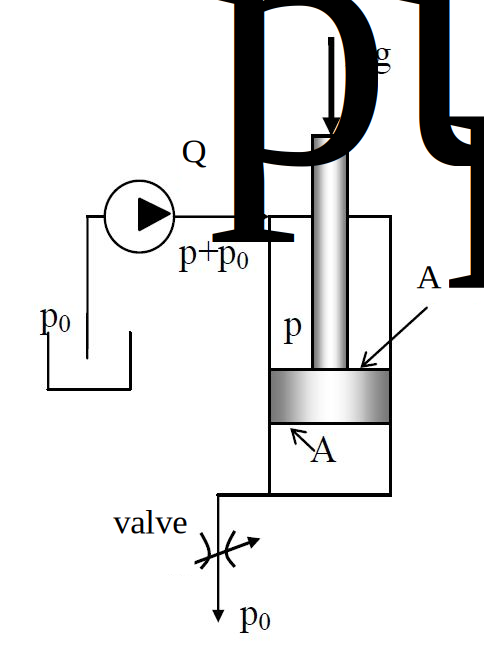
\includegraphics[width=0.4\textwidth]{Problem_solving/figs/cylinder-problem.png}
\end{wrapfigure}

The two areas:
\begin{align*}
A_{ring} = \frac{\pi}{4} (D^2-d^2) = 0.001348~\mathrm{m^2}\\
A = \frac{\pi}{4} D^2 = 0.001964~\mathrm{m^2}.
\end{align*}

Newton's law:
%\begin{align*}
%A(p_0+\Delta p_{valve}) = A_{ring}p + mg = A_{ring}(p_0 + \Delta p) + mg + A_{piston}p_0 = Ap_0 + A_{ring} \Delta p + mg.
%\end{align*}
\begin{multline*}
A(p_0+\Delta p_{valve}) = A_{ring}p + mg = \\
A_{ring}(p_0 + \Delta p) + mg + A_{piston}p_0 = Ap_0 + A_{ring} \Delta p + mg.
\end{multline*}

Continuity equation for the upper part of the cylinder:
\begin{align*}
Q_{pump} = A_{ring}v = 0.001347~\mathrm{m^2}\cdot 0.064~\frac{\mathrm{m}}{\mathrm{s}} = 5.176~\frac{\mathrm{dm^3}}{\mathrm{min}}.
\end{align*}

Pressure from the performance curve of the pump:
\begin{align*}
\Delta p = \frac{8.6-Q_{pump}}{0.0467} = \frac{8.6-5.176}{0.0467} = 73.3~\mathrm{bar}.
\end{align*}

Continuity equation for the valve:
\begin{align*}
Q_{valve} = Av = 0.001964~\mathrm{m^2}\cdot 0.064~\frac{\mathrm{m}}{\mathrm{s}} = 7.54~\frac{\mathrm{dm^3}}{\mathrm{min}}.
\end{align*}

Bernoulli's equation for the valve: 
\begin{align*}
Q_{valve} = \mu A_{valve}\sqrt{\frac{2}{\rho_{oil}}\Delta p_{valve}}.
\end{align*}

Rearranging Newton's law yields
\begin{align*}
\Delta p_{valve} = \frac{A_{ring}\Delta p + mg}{A} = \frac{0.001348\cdot 7.33\cdot 10^6 + 700\cdot 9.81}{0.001964} = 85.27~\mathrm{bar}, 
\end{align*}
and finally,
\begin{align*}
A_{valve} = \frac{Q_{valve}}{\mu \sqrt{\frac{2}{\rho_{oil}}\Delta p_{valve}}} = \frac{0.0001257}{0.7\cdot \sqrt{\frac{2}{970}\cdot 85.27\cdot 10^5}} = 1.354~\mathrm{mm}.
\end{align*}

The useful power of the pump is
\begin{align*}
P_{p,u}=Q_{pump}\Delta p_{pump} = (8.6-0.0467 \Delta p)\Delta p.
\end{align*}

The criterion for the local maximum is $\frac{\mathrm{d}P_{p,u}}{\mathrm{d}\Delta p} = 8.6-2\cdot 0.0467\cdot \Delta p_{opt} = 0 \rightarrow \Delta p_{opt} = 92.1~\mathrm{bar}$. At this operating point, $Q_{opt}=4.3~\frac{1}{\mathrm{min}}$, and $P_{p,u,max} = 660~\mathrm{W}$.
